\documentclass[border=5pt]{article}
\usepackage[margin=0.7in]{geometry}
\pagestyle{empty}
\usepackage{tikz}
\usetikzlibrary{arrows.meta,positioning}

\begin{document}
\begin{center}
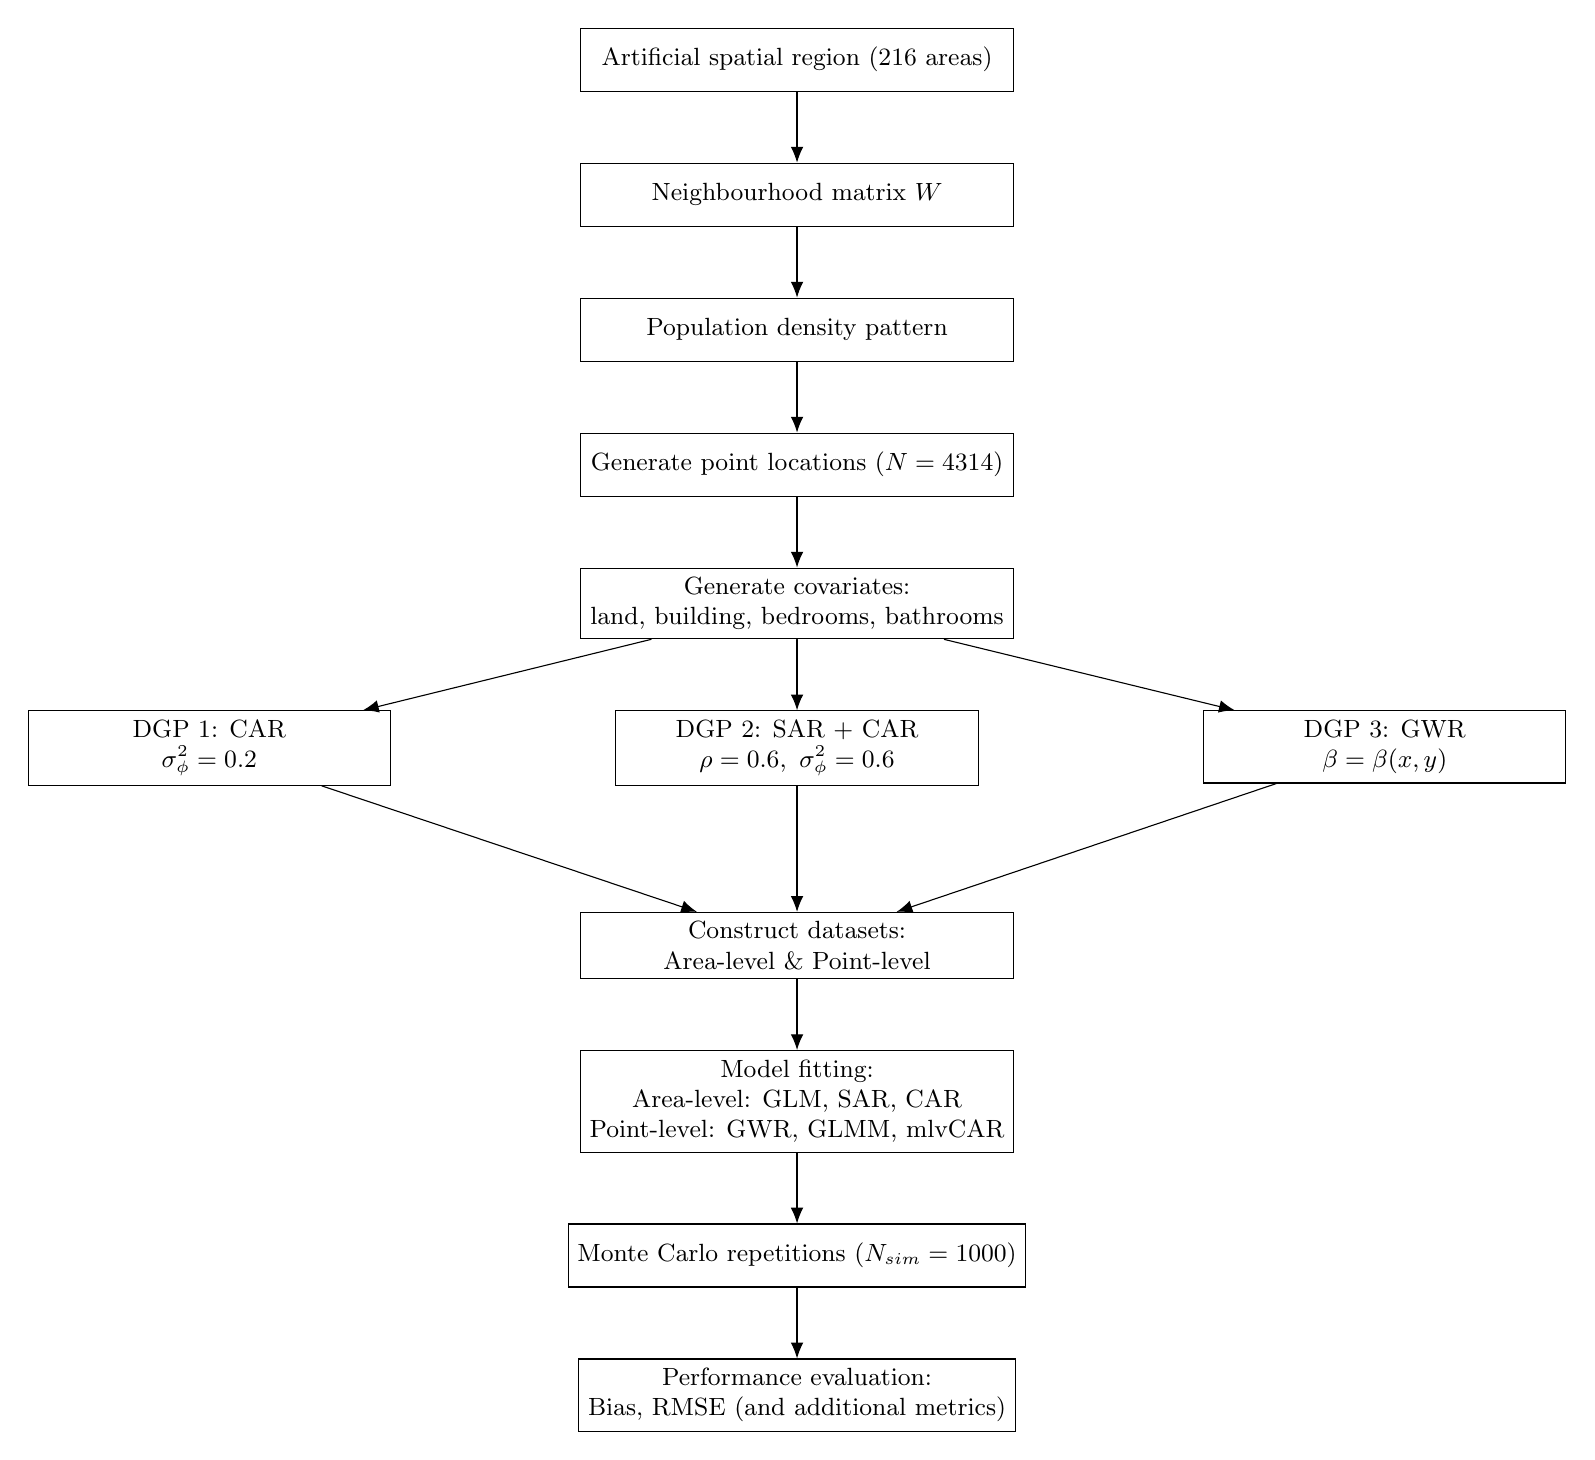
\begin{tikzpicture}[
  node distance=9mm and 14mm,
  >=Stealth,
  block/.style={rectangle,draw,align=center,minimum width=55mm,minimum height=8mm},
  smallblock/.style={rectangle,draw,align=center,minimum width=46mm,minimum height=8mm},
  font=\small
]

\tikzset{
  connect/.style={-{Latex[length=2mm,width=1.6mm]}, line cap=round}
}

% --- Data construction ---
\node[block](region){Artificial spatial region (216 areas)};
\node[block,below=of region](W){Neighbourhood matrix $W$};
\node[block,below=of W](dens){Population density pattern};
\node[block,below=of dens](pts){Generate point locations ($N=4314$)};
\node[block,below=of pts](covs){Generate covariates:\\land, building, bedrooms, bathrooms};

\draw[connect] (region) -- (W);
\draw[connect] (W) -- (dens);
\draw[connect] (dens) -- (pts);
\draw[connect] (pts) -- (covs);

% --- DGPs ---
\node[smallblock,below left=of covs,xshift=-10mm](car){DGP 1: CAR\\$\sigma^2_\phi=0.2$};
\node[smallblock,below=of covs](sarcar){DGP 2: SAR + CAR\\$\rho=0.6,\ \sigma^2_\phi=0.6$};
\node[smallblock,below right=of covs,xshift=10mm](gwr){DGP 3: GWR\\$\beta=\beta(x,y)$};

\draw[connect] (covs) -- (car);
\draw[connect] (covs) -- (sarcar);
\draw[connect] (covs) -- (gwr);

% --- Data structure split ---
\node[block,below=16mm of sarcar](split){Construct datasets:\\Area-level \& Point-level};

\draw[connect] (car) -- (split);
\draw[connect] (sarcar) -- (split);
\draw[connect] (gwr) -- (split);

% --- Model fitting ---
\node[block,below=of split](models){
Model fitting:\\
Area-level: GLM, SAR, CAR\\
Point-level: GWR, GLMM, mlvCAR
};

\draw[connect] (split) -- (models);

% --- Simulation loop ---
\node[block,below=of models](loop){Monte Carlo repetitions ($N_{\text{sim}} = 1000$)};

\draw[connect] (models) -- (loop);

% --- Evaluation ---
\node[block,below=of loop](metrics){
Performance evaluation:\\
Bias, RMSE (and additional metrics)
};

\draw[connect] (loop) -- (metrics);

\end{tikzpicture}
\end{center}
\end{document}